\subsection{COW quality control}

\begin{frame}
  {DECOW and ENCOW 14\slash 16: Example of improvements to annotation quality}
  \begin{itemize}
    \item 3,866 manual additions to TreeTagger lexicon (DE)
    \item two-pass tagging with lemmatization of unknown items by SMOR (DE)
    \item Dependency parses from IMS Stuttgart (by FU Berlin for EN)

	\vspace{0.5cm}

    \item Named entities (DE, EN)

    \begin{itemize}
		\item NER quality for DE evaluated by Lea Helmers (HU Berlin)
		\item quality depended highly on register
		\item standard written: $prec=0.76$ $rec=0.56$
		\item spontaneous written: $prec=0.53$ $rec=0.32$
      \end{itemize}
  \end{itemize}
\end{frame}



\begin{frame}
  {DECOW14A: TreeTagger and Mate-Morphology}
  Post-hoc evaluation of 10.000 tokens (from sentences):\\
  TreeTagger was excellent, Mate morphology horrible, replaced by Marmot
  \vspace{0.5cm}
  \begin{center}
    \scalebox{0.8}{
      \begin{tabular}[h]{lrrrrrrrr}
	\hline
	   & POS & Case & Num & Gend & Comp & Per & Tense & Mod \\
	\hline
	\hline
	correct $\approx$ & 0.97 & 0.83 & 0.9 & 0.79 & 0.9 & 0.9 & 0.87 & 0.83 \\
	\hline
      \end{tabular}
    }
  \end{center}
 
\end{frame}


%\begin{frame}
%	{Evaluation nach Leipziger Art: Satzlängen}
%	\centering
%	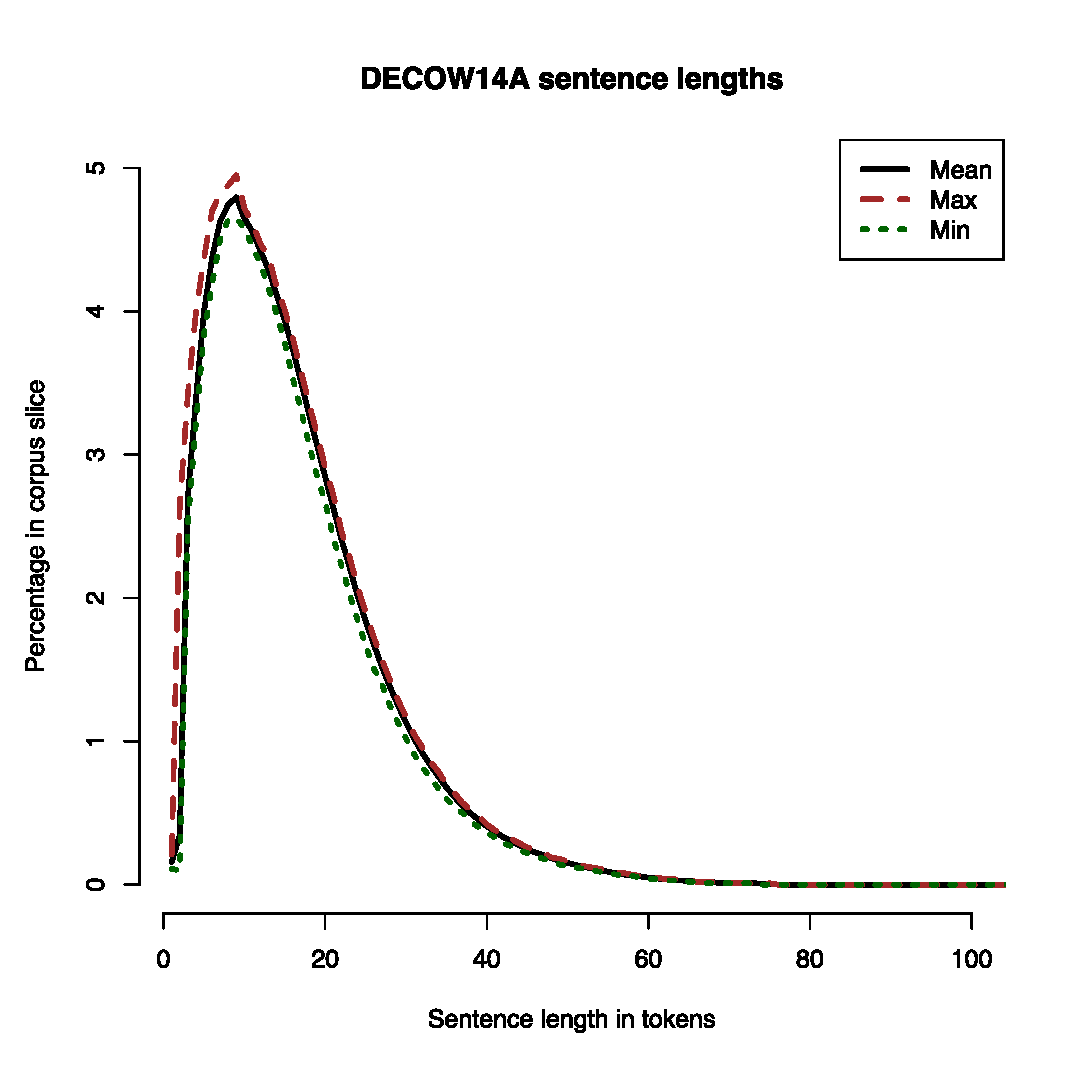
\includegraphics[height=0.8\textheight]{graphics/s_de}
%\end{frame}
%
%\begin{frame}
%	{Evaluation nach Leipziger Art: Satzlängen}
%	\centering
%	\includegraphics[height=0.8\textheight]{graphics/s_en}
%\end{frame}
%
%\begin{frame}
%	{Evaluation nach Leipziger Art: Satzlängen}
%	\centering
%	\includegraphics[height=0.8\textheight]{graphics/s_es}
%\end{frame}
%
%\begin{frame}
%	{Evaluation nach Leipziger Art: Satzlängen}
%	\centering
%	\includegraphics[height=0.8\textheight]{graphics/s_nl}
%\end{frame}
%
%\begin{frame}
%	{Evaluation nach Leipziger Art: Satzlängen}
%	\centering
%	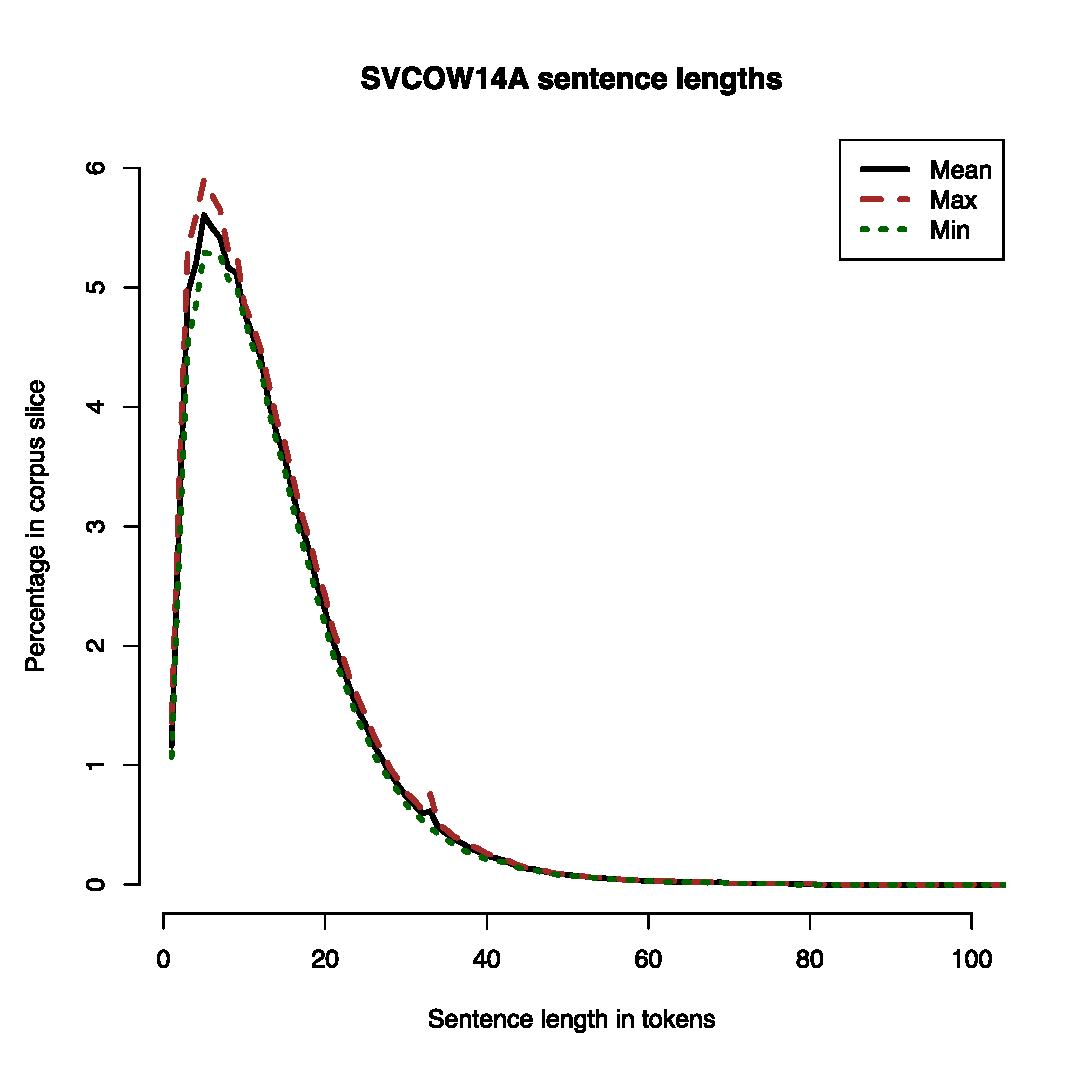
\includegraphics[height=0.8\textheight]{graphics/s_sv}
%\end{frame}

